\chapter{Trust Model Design}
\label{ch:trust-model-design}
In this chapter, we will describe how we approached problems of trust in global peer-to-peer environment in section \ref{sec:computational-model},how can we evaluate single interaction between two peers in section \ref{sec:interaction-evaluation-strategies}, how we mitigate cold start problem \ref{sec:cold-start-problem} and finally, how do we aggregate network threat intelligence into a single network opinion in section \ref{sec:network-intelligence-aggregation}.

Our trust model, Fides, operates in four phases, first it receives data, then it aggregates the data, evaluates the interactions with each peer and as a last step it updates the service trust for the next interaction.
See figure \ref{fig:trust-model-life-cycle}, where is this process visualized.

\begin{figure}[ht!]
    \centering
    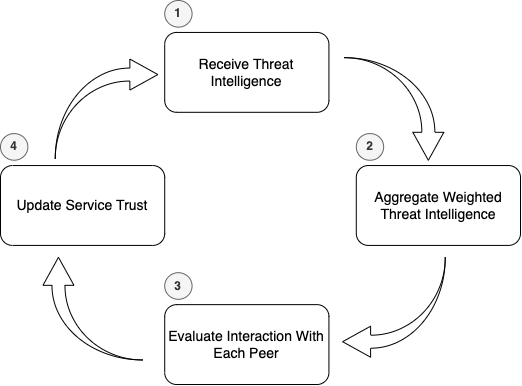
\includegraphics[width=0.7\textwidth]{assets/service_trust_diagram.png}
    \caption{Trust Model Life Cycle}
    \label{fig:trust-model-life-cycle}
\end{figure}

In the following sections we will be using this terminology and words when talking about the trust model.

\begin{itemize}
\item \textbf{service trust} - how much a trust model trust a peer to provide us a good service - it is not necessarily how much we trust the data we received from the peer as to the final computation we may include the information about peer's IP address from the Slips (what does Slips think about the IP address)
\item \textbf{target} - an IP address or domain - point of interest that can be source of network traffic and Slips has a capability to assign threat intelligence data to this object
\item \textbf{remote peer} - peer that is running somewhere on the internet and it is connected to the global peer-to-peer network
\item \textbf{local peer} - local instance of Slips that is connected to the global peer-to-peer network and runs instance of Fides
\end{itemize}

\section{Computational Model of Fides}
\label{sec:computational-model}
This section describes how does Fides come up with a single most important value $st_{i,j}$ service trust. Service trust describes how much can local peer $i$ trust remote peer $j$.
Used algorithm, that computes $st_{i,j}$, is based on SORT\cite{sort} with modifications to fit our use case - a global peer-to-peer network for sharing threat intelligence. The modifications are based on the interaction evaluation strategies proposed in \ref{subsec:interaction-evaluation} and algorithms to solve cold start problem described in \ref{subsec:cold-start-problem}.

\subsection{Intuition}
In the following pages, we describe the process top-down starting with the most important parts - service trust - and then breaking it down to bits.
There are two main ideas behind the most of the equations. 

The first one is that we want to robustly capture average behavior of the peers. In order to do that, we will be computing average behavior and standard deviations from said behavior and normalizing them.

Secondly, we will be comparing and weighting first hand experience with the remote experience. 
First hand experience is what happened between local and remote peer during time they interacted. This can be, for example, threat intelligence sharing, file sharing or the results of recommendation protocol.
Remote experience is what happened between one remote peer and another remote peer. In other words, first hand experience for peer $j$ are actions between $j$ and $z$. When $j$ shares information about these action with peer $i$, for $i$ it is a remote experience.

\begin{table}[ht]
\centering
\begin{tabular}{ c | m{20em} }
 $i$ & local peer, instance of Fides \\
 \hline
 $j$ & remote peer somewhere on the internet \\
 \hline
 $st_{i, j}$ & service trust - how much $i$ trusts $j$ that it provides good service \\
 \hline
 $r_{i, j}$ & $i$'s reputation value about $j$ \\
 \hline
 $rt_{i, j}$ & $i$'s recommendation trust about $j$ \\
 \hline
 $sh_{i, j}$ & size of $i$'s service history with $j$ \\
 \hline
 $s^{k}_{i, j}$ & $i$'s satisfaction value with interaction with peer $j$ in window $k$\\
 \hline
 $w^{k}_{i, j}$ & weight of $i$'s interaction with $j$ in $k$ \\
 \hline
 $f^{k}_{i, j}$ & fading effect of $i$'s interaction with $j$ in $k$ \\
\end{tabular}
\caption{Fides Computational Model Notation}
\label{tab:notation-computational-model}
\end{table}

\vspace{5mm}

\noindent 
The table \ref{tab:notation-computational-model} describes the most important notation we use in the following sections.

\subsection{Service Trust}
One of the major goals of the algorithm is to compute the service trust $st_{i,j}$.
We do that by weighting local experience with peer's $j$ service, with the reputation, $j$ got when it connected to the $i$. The weight here is size of the service interaction history $sh_{i,j}$ to maximal history size $sh_{max}$.

\begin{equation}\label{eq:service-trust}
st_{i,j}=\frac{sh_{i,j}}{sh_{max}} \cdot \left(cb_{i,j} - \frac{1}{2} \cdot ib_{i,j} \right) +\left(1-\frac{sh_{i,j}}{sh_{max}}\right) \cdot r_{i,j}
\end{equation}

The equation implies that the more interaction there was, between $i$ and $j$, the bigger impact on $st_{i,j}$ it has. 
In other words, the more $i$ and $j$ interact the less $i$ rely on the reputation that $i$ computed from the values provided by the network, at the time when $j$ was seen for the first time.

First part of the equation contains $cb_{i,j}$ - \textit{competence belief} - and $ib_{i,j}$ - \textit{integrity belief}. \textit{Competence belief} represents how well $j$ satisfied the $i$ with the past interactions. We measure it as an average of interactions from the past.
\textit{Integrity belief} is a level of confidence in predictability of future interactions. $ib_{i,j}$ is then measured as deviation from the average behavior $cb_{i,j}$. \cite{sort}

In order to mitigate cold start problem outlined in \ref{subsec:cold-start-problem} and in cases when there are no or little interactions between $i$ and $j$, the algorithm relies on $r_{i,j}$ - reputation value.

\subsection{Interaction Evaluations}
\label{subsec:interaction-evaluation}
In order to determine what remote peers are providing valuable data and what peers are are not, the local peer needs to be able to evaluate each interaction it had with the remote peer.
In general, there are two options how to approach this - either by designing evaluation that is protocol aware (meaning, that it understands the protocol and the data that are two peers sharing with each other), or by having an evaluation function that does not need to understand the protocol and can be used for any data.

We choose to implement both approaches and they are described in the following sections. In order to evaluate which strategy is better in what scenarios, we designed and run many simulations - their results are described in section \ref{sec:simulations-and-evaluations}.

% TODO: maybe do not use S and C when referring to score and confidence as we use "s" for satisfaction
We will use notation from table (\ref{table:interaction-eval})  when referring to peers and their interactions.
\begin{table}[h!]
\centering
\begin{tabular}{ c | m{20em} }
 $i$ & local peer \\
 \hline
 $j$ & remote peer \\
 \hline
 $T$ & target of network intelligence, domain or IP address \\
 \hline
 $k$ & evaluation window \\
 \hline
 $s^{k}_{i, j}$ & $i$'s satisfaction value with interaction with peer $j$ in window $k$\\
 \hline
 $S^{k}_{j, T}$ & score computed by the peer $j$ about target $T$ in window $k$ \\
 \hline
 $C^{k}_{j, T}$ & confidence, how much is the score correct \\
 \hline
 $S^{k}_{T}$ & aggregated score from all threat intelligence reports in window $w$ for target $T$ \\
 \hline
 $C^{k}_{T}$ & aggregated confidence
\end{tabular}
\caption{Interactions Symbols}
\label{table:interaction-eval}
\end{table}


\subsubsection{Evaluate all interactions with the same value}
\label{subsubsec:same-eval-for-all-interactions}
The strategy, that does not need to understand underlying data, their semantics nor their structure.
It is a naive approach when the trust model uses the same satisfaction value for all data it received. It does not check, if the data make sense (for example when all other peers but one are reporting that the IP address is malicious) and assigns all peers same satisfaction value $s^{k}_{i, j}$. 
The idea behind this algorithm is that when the peers are interacting for a longer time or have more interactions, they're more trustworthy.

This approach is for example used by the botnet \textbf{Sality} or by the \textbf{Dovecot} trust model. Fides implements it as $EvenTIEvaluation$ strategy with configurable satisfaction value and administrator can use this strategy if they see it as the most optimal.

The disadvantage of this approach is, that we do not penalize remote peers when they provide wrong data, because the evaluation method does not care nor understand the underlying data.
Because of that and in a case when the adversary gains the service trust of the model by following the protocol for longer time, it may significantly influence the aggregated score as the adversary has higher trust then other remote peers. If this happens, there is no way to automatically downgrade adversary's service trust.

\subsubsection{Use aggregated network intelligence for evaluation}
\label{subsub:distance-based-eval}
Because Fides is designed for the sharing and aggregating threat intelligence and understands the protocol that is being used, we can utilize this and penalize peers that are providing local peer with incorrect data.
The interaction evaluation is performed at the end of the threat intelligence sharing process, at that point, Fides already aggregated data and decided what is the aggregated network score and confidence. 
Thus, we can utilize aggregated values and use it as a base line. Then we compare it against every each remote peer's threat intelligence we received. This evaluation strategy is implemented in the Fides a as a $DistanceBasedTIEvaluation$.

% TODO: here we need to set correct indexes, because k-th interaction between local and peer i is not necessarily the same number as for the peer i+1 -> that means that for S_a we will need another number
% TODO: we need to move this to another section and to describe what is score and what is confidence
Suppose, that remote peer $j$ provided data about target $T$ to local peer $i$ in window $k$. Provided data consist of score and confidence - ($S^{k}_{j, T}$, $C^{k}_{j, T}$). Where score,  $-1 \leq S^{k}_{j, T} \leq 1$, indicates if the target is malicious ($-1$) or begin ($1$). The confidence $0 \leq C^{k}_{j, T} \leq 1$ on the other hand indicates, how much is the peer sure about its assessment of $S^{k}_{j, T}$.

In order to evaluate interaction between the local peer $i$ and remote peer $j$ we need to compute satisfaction value $s^{k}_{i, j}$. 
It holds that  $0 \leq s^{k}_{i, j} \leq 1$ - where $1$ means peer $i$ was satisfied with the interaction.
% TODO: [?] this equation can be more robust, we can for example, compute standard deviation from the S^{k}_{T} and then compare each S to nearest second quantile -> that way the equation is more robust
\begin{equation}
s^{k}_{i, j} = \left(1 - \frac{|{S}^{k}_{T} - S^{k}_{j, T}|}{2} \cdot C^{k}_{j, T}\right) \cdot C^{k}_{T}
\end{equation}

Where $S^{k}_{T}$ is final score aggregated across the reports from the peers, $C^{k}_{T}$ is aggregated confidence.

The problem in this evaluation algorithm are the situations when the aggregated confidence $C^{k}_{T}$ is close to $0$. In this case the algorithm will penalize all peers for providing any threat intelligence as the final $s^{k}_{i, j}$ is close to $0$. Another issue with this approach is that when a single honest peer has a unique information about an IP address or domain, which is significantly different then what other peers have, it is automatically penalized for not sharing the same opinion as the other peers. However, if the peer is trusted enough, it has higher impact on the aggregated value and it is not penalized too much.

\subsubsection{Use network intelligence only if the confidence is high enough}
\label{subsubsec:network-intelligence-conf-high-enough}
In order to compensate for the low confidence $C^{k}_{T}$ and penalizing all peers in algorithm explained in \ref{subsub:distance-based-eval}, this evaluation strategy considers $C^{k}_{T}$ value and employs  $DistanceBasedTIEvaluation$ only when the  $C^{k}_{T}$ is \textit{"high enough"}. In this case \textit{"high enough"} means higher then configured value by the Slips administrator - ${CT}$.
In a case when  $C^{k}_{T} < {CT}$, the algorithm fall backs to using $EvenTIEvaluation$, because it is not possible to distinguish between \textit{"good"} and \textit{"bad"} network intelligence due to low confidence of the decision. 
This strategy is implemented in Fides under the name $ThresholdTIEvaluation$.

% TODO: I'm not sure if we really need this schema
\begin{algorithm}
\caption{$ThresholdTIEvaluation$}\label{alg:threshold-ti-evaluation}
\begin{algorithmic}[1]
\State ${CT} \gets configuration$ \Comment{configuration provided by the administrator}
\If{$C^{k}_{T} < {CT}$}
	\State $s^{k}_{i, j} \gets EvenTIEvaluation()$
\Else
    \State $s^{k}_{i, j} \gets DistanceBasedTIEvaluation()$
\EndIf
\end{algorithmic}
\end{algorithm}

\noindent What should be the correct value for $CT$ from configuration is subject to evaluation in the simulations in section \ref{sec:simulations-and-evaluations}.

\subsubsection{Use local threat intelligence to evaluate network intelligence}
\label{subsub:use-local-threat-to-evaluate}
This approach uses similar equation for computing satisfaction value outlined in \ref{subsub:distance-based-eval}. However, the input is different - instead of comparing remote peer's ($j$ ) threat intelligence ($S^{k}_{j, T}$, $C^{k}_{j, T}$) to aggregated intelligence ($S^{k}_{T}$, $C^{k}_{T}$), we compare it to the threat intelligence of the local ($i$) Slips instance - ($S^{k}_{i, T}$, $C^{k}_{i, T}$). Thus the evaluation is following:

\begin{equation}
s^{k}_{i, j} = \left(1 - \frac{|{S}^{k}_{i, T} - S^{k}_{j, T}|}{2} \cdot C^{k}_{j, T}\right) \cdot C^{k}_{i, T}
\end{equation}

This approach is useful when local peer has enough information about the target, but it wants to verify the behavior of the remote peers.
To determine whether they are sending data that are somewhat correct. This strategy is implemented in Fides with name $LocalCompareTIEvaluation$.

\subsubsection{Weight local opinion with aggregated one}
Another implemented strategy combines \ref{subsub:distance-based-eval} and \ref{subsub:use-local-threat-to-evaluate} and mixes them using weight $w$, provided from the configuration.
This is good approach when the the Slips or the network has a lot of data on the target. It evaluates interactions with what local instance thinks and what the network opinion is.
What the correct mixture is is subject to simulations and configuration from the administrator.

\begin{equation}
\begin{split}
    s^{k}_{i, j} = w &\cdot \left(1 - \frac{|{S}^{k}_{i, T} - S^{k}_{j, T}|}{2} \cdot C^{k}_{j, T}\right) \cdot C^{k}_{i, T} + \\
    (1-w) &\cdot \left(1 - \frac{|{S}^{k}_{T} - S^{k}_{j, T}|}{2} \cdot C^{k}_{j, T}\right) \cdot C^{k}_{T}
\end{split}
\end{equation}

\noindent
In Fides implemented as the $WeightedDistanceToLocalTIEvaluation$.

\subsubsection{Utilize all available data in evaluation}
The goal of this strategy is to evaluate the received data with as much confidence as possible while having fully automatic process without the administrator's configuration.
In order to do that, we combine all previous strategies into one, where we utilize all available information into a single $s^{k}_{i, j}$ value.

We introduce new variables here - $p_{0}, p_{1}, p_{2}$ - which are essentially weights of the particular strategies. These weights are based on the confidence, that the strategy has in its own decision.
Note, that there is a hierarchy and order matters. 
In our case we decided to prefer decisions coming from strategy \ref{subsub:distance-based-eval}, then we add data from the \ref{subsub:use-local-threat-to-evaluate} and if the final decision still does not have confidence of $1$, we add static value configured by the administrator (noted as $S_{C}$). 
The last part - $S_{C}$ - simulates static strategy described in \ref{subsubsec:same-eval-for-all-interactions} and is set by the Slips administrator.
% TODO should we use min or the detailed version?

\begin{equation}
\label{equation:strategies-weights}
\begin{split}
    p_{0} &= {C}^{k}_{T} \\
    p_{1} &= \frac{1 - {C}^{k}_{T} + {C}^{k}_{i, T} - |1 - {C}^{k}_{T} - {C}^{k}_{i, T}|}{2} \\
    p_{1} &= min(1 - {C}^{k}_{T}, {C}^{k}_{i, T}) \\
    p_{2} &= 1 - p_{0} - p_{1}
\end{split}
\end{equation}
The weights $p_{0}, p_{1}, p_{2}$ in \ref{equation:strategies-weights}, are designed to gather as much confidence as possible. $p_{0}$ is confidence of the aggregated network data, essentially saying how much is the network sure about the given score. 
$p_{1}$ is the confidence coming from the local IPS and the $p_{2}$ is the remaining confidence to $1$.

When we have the weights, we can compute final $s^{k}_{i, j}$ where we use strategies - $p_{0} \cdot \ref{subsub:distance-based-eval}$, $p_{1} \cdot \ref{subsub:use-local-threat-to-evaluate}$ and $p_{2} \cdot \ref{subsubsec:same-eval-for-all-interactions}$. 
\begin{equation}
\begin{split}
    s^{k}_{i, j} &= \\
    &p_{0} \cdot \left[\left(1 - \frac{|{S}^{k}_{T} - S^{k}_{j, T}|}{2} \cdot C^{k}_{j, T}\right) \cdot C^{k}_{T}\right] + \\
    &p_{1} \cdot \left[\left(1 - \frac{|{S}^{k}_{i, T} - S^{k}_{j, T}|}{2} \cdot C^{k}_{j, T}\right) \cdot C^{k}_{i, T}\right] + \\
    &p_{2} \cdot S_{C}
\end{split}
\end{equation}

\noindent
This strategy is implemented in Fides under a name $MaxConfidenceEvaluation$.


\section{Cold Start Problem}
\label{sec:cold-start-problem}
A dynamic and global environment such as a global peer-to-peer network is open to anyone since any peer can freely join and leave. Because of that, the local peer will encounter many other peers that were not seen before. Therefore, the trust model does not have any information about their reliability or how much it can trust them. 
New benign peers need to be \textit{somehow} trusted by the local peer in order to be a useful part of the network. However, the local peer also needs to be able to discover new malicious peers that are trying to gain its trust.

The problem of how to know something about a new entity in order to quickly work better is called the \textit{Cold Start Problem}~\cite{christensen2014hybrid}. For Fides it means how to compute a good initial trust for new unknown peers. 

We selected several solutions to this issue, which are all implemented in Fides. Fides also combines them according to a provided configuration with the aim to achieve the best result for the cold start problem with adversarial peers.

\subsection{Static Initial Trust}
\label{subsec:static-initial-trust}
In this approach, whenever the trust model encounters a new peer, it assigns a static value as an initial trust. The value is assigned by pre-choosing some third-party trust models in the configuration.

For example, in the \textbf{Dovecot} trust model~\cite{dita}, every peer starts with trust $1$ (highest possible), and various interactions can lower the trust in the peer to $0$. In other words, the trust model considers new peers honest from the beginning, and only during this time their reputation can be lowered when they perform incorrect interactions or are discovered as a malicious peer.

On the other hand, the \textbf{Sality} botnet~\cite{falliere2011sality} uses a value called \textit{goodcount} as a counter of good interactions with any other peer, the larger the \textit{goodcount}, the greater trust the local peer has on the remote peer. The goodcount for each new peer starts with $0$ in Sality. Meaning, that the botnet does not trust fresh peers at all and they can gain trust only by following the Sality protocol.

The model of \textit{static initial trust} is easy to implement, but it requires assumptions about the network. If the network is considered \textit{mostly benign}, it might be safe to use an initial trust of $1$, however for highly adversarial networks using an initial trust of $1$ might be dangerous and it is better to use $0$. 
Using low initial trust and no mechanism how to gain more trust fast means, that the benign peers that joined recently, don't affect the final decisions of the model even though they might have useful information about adversaries.

Static initial trust is supported by Fides as a form of fallback when no other cold start technique is used. The administrator provides a configuration that contains the initial reputation for each new peer.

\subsection{Pre-Trusted Peers}
\label{subsec:pre-trusted-peers}

This master thesis was done simultaneously to the master thesis on global P2P security TI sharing by Bc. Martin Řepa~\cite{nl} which implements the new idea of pre-trusted peers in organizations for the Slips IPS. Therefore, we worked with the concept of pre-trusted organizations which have pre-trusted peers. In this case, Fides can use this knowledge and assign a higher or lower trust to new peers.

The global P2P framework implemented by Řepa supports these type of peers and provides a cryptographically-secure way how to identify a single peer in the network, and its membership in an organization.
This allows Fides to \textit{pre-trust} specific peers or all the peers from organizations by assigning them an initial value.

Fides can be configured to use pre-trust in two different ways. First, to assign the pre-trusted peers an initial \textit{reputation}. This means that the peer will have an initial reputation, but it will be required to interact with the local peer and it will slowly change that initial reputation according to its interactions with others. All the interactions will be evaluated and Fides will compute a service trust for the peer, as described in Section~\ref{sec:interaction-evaluation-strategies}. 

Second, Fides can use the initial pre-trusted value read from the configuration as the final service trust. This effectively means that Fides will not evaluate any data received from the pre-trusted peer and this service trust will be kept forever. 

This configuration for the Fides is called \textit{enforceTrust}, if it is enabled and thus $enforceTrust = False$ is set in the configuration, Fides uses first variant where the trust for the peer will move during the interactions. When administrator uses $enforceTrust = True$, Fides uses second option and fixates the service trust for the peer to a set \textit{pre-trust}.

Both options helps to solve the cold start problem for specific peers and organizations, as they will start with a high reputation or fixed service trust. Which organization or peer to trust is completely left to the administrator of Slips. 
The inspiration for which organization or to which peer to trust provides, for example, Tor and their directory authorities~\cite{torauth}. However as the administrator needs to know the identity of the peers or organization, it does not solve the cold start problem globally for all peers.

\subsection{Recommendations}
\label{subsec:recommendations}
As the local peer might have multiple remote peers that it trusts enough, Fides uses these relationships to ask the remote peers about how much they trust a new peer. Fides only asks for recommendations when the local peer finds a new peer.  

The recommendation system introduces new attack vectors, that can be exploited by adversaries either by getting trust for the malicious peer or by lowering trust in honest peers that might have some threat intelligence about the malicious actor. 
These attacks are called \textit{bad-mouthing} and \textit{unfair praises} and we need to consider them and implement countermeasures.

Because of the possible attacks, the local peer should not solely rely on the network recommendations when computing the final service trust for the fresh peer. In case, when the recommending peers are malicious, it might skew the decisions of the local peer for the time being.
In order to solve this, when computing the final service trust for the remote peer, the local peer should take into account its own interaction with the peer as well as the received recommendations.

Moreover, the local peer should request recommendations only if it has \textit{enough} trusted remote peers, otherwise, it can expose itself to \textit{bad-mouthing} and \textit{unfair praises} attacks more easily.

\vspace{7mm}

Fides employs recommendation systems based on SORT~\cite{sort} and combines it with the pre-trusted peers~(\ref{subsec:pre-trusted-peers}) as well as with the static initial trust~(\ref{subsec:static-initial-trust}) as a fallback when no other option is available due to constraints such as having not enough trusted peers.
The algorithm used for the recommendation system is explained in detail in the section~\ref{sec:computational-model}.

\section{Network Intelligence Aggregation}
\label{sec:network-intelligence-aggregation}
Fides is a trust model designed for global peer-to-peer networks of Slips instances.
It is designed to support Slips in detecting malicious actors on the network and enables threat intelligence sharing between peers of Slips instances.
Because Slips was designed to be as modular as possible, Fides is effectively running as a module that provides aggregated threat intelligence to Slips. 
In other words, Fides provides a view of what the network thinks about some threat intelligence target. This is necessary so Slips can have a unique \textit{view} of the network on a specific Threat Intelligence.
Fides needs to aggregate elements of threat intelligence from remote peers into a single value that is then presented to Slips.

Fides needs to say that some reports are better than others, based on the service trust the local peer has in the remote peer (previously computed as $st^{k}_{i, j}$).
Thus Fides needs to weigh every report based on this trust and come up with an aggregated score $S^{k}_{T}$.
Apart from the aggregated score, Fides needs to compute the aggregated confidence $C^{k}_{T}$ that expresses how confident $i$ is about the aggregated score $S^{k}_{T}$ that was computed in the previous step.

Once aggregated, the computed score and confidence ($S^{k}_{T}$, $C^{k}_{T}$) are sent to Slips to report data on target $T$.
Apart from sending to Slips, these same values can be also used to evaluate the interaction of the remote peers, depending on the selected interaction evaluation strategy. We describe this more in depth in Section~\ref{sec:interaction-evaluation-strategies}.

We designed and implemented two different functions for aggregating threat intelligence and computing $S^{k}_{T}$ alongside with $C^{k}_{T}$.
Both of them are implemented in Fides under their respective names and which method performs better under what circumstances is a subject of the experiments in Chapter~\ref{ch:experiments}.

\subsection{AverageConfidenceTIAggregation}
\label{subsec:AverageConfidenceTIAggregation}

In this method, the aggregated score $S^{k}_{T}$ is the sum of $S^{k}_{j, T}$, which is the score sent by each peer $j$ about target $T$ in time window $k$; weighed with the normalized service trust that $i$ computed for peer $j$, denoted $wst^{k}_{i, j}$. The sum is done over the set of remote peers that provided a report to $i$ for $T$ in time window $k$, denoted $R^{k}_{i, T}$. We calculate it in Equation~\ref{eq:ti_aggregation_score}.

\begin{equation}
\begin{split}
    S^{k}_{T} &= \sum_{{j}\in R^{k}_{i, T}} wst^{k}_{i, j} \cdot S^{k}_{j, T}
\end{split}
\label{eq:ti_aggregation_score}
\end{equation}

\noindent
The normalized service trust $wst^{k}_{i,j}$ used as weight is computed as:

\begin{equation}
\begin{split}
    wst^{k}_{i,j} &= \frac{1}{\sum_{{j}\in R^{k}_{i, T}} st^{k}_{i, j}} \cdot st^{k}_{i, j} \\
\end{split}
\label{eq:normalized_service_trust_ti_aggregation}
\end{equation}

\noindent
Equation~\ref{eq:normalized_service_trust_ti_aggregation} estimates the percentage that the service trust on $j$ $st^{k}_{i, j}$ has relative to the total sum of service trust received by $i$ for all peers, for this target $T$, in time window $k$.

We compute the aggregated confidence $C^{k}_{T}$ for this strategy as:

\begin{equation}
\begin{split}
    C^{k}_{T} &= \frac{1}{|R^{k}_{i, T}|} \cdot \sum_{{j}\in R^{k}_{i, T}} st^{k}_{i, j} \cdot C^{k}_{j, T}
\end{split}
\end{equation}

\noindent
Which is an average over all the peers that sent to $i$ a report on $T$ in time window $k$, of the weighted confidence sent by peer $j$ on target $T$ on time window $k$. The weight is done by the service trust that $i$ has on $j$ on time window $k$.


\subsection{WeightedAverageConfidenceTIAggregation}
\label{subsec:WeightedAverageConfidenceTIAggregation}

This strategy uses Equation~\ref{eq:ti_aggregation_score} to compute the aggregated score $S^{k}_{T}$ similarly to the $AverageConfidenceTIAggregation$ in Section~\ref{subsec:AverageConfidenceTIAggregation}.
However, the way how this strategy calculates $C^{k}_{T}$ is different. 
Instead of using the service trust $st^{k}_{i, j}$ to determine the correct trust in the confidence $C^{k}_{j, T}$ submitted by peer $j$ and then diving it by the number of peers, it uses the normalized service trust $wst^{k}_{i,j}$ computed in Equation~\ref{eq:normalized_service_trust_ti_aggregation} that already contains the weight of the peers in the final decision.

\begin{equation}
\begin{split}
    C^{k}_{T} &= \cdot \sum_{{j}\in R^{k}_{i, T}} wst^{k}_{i,j} \cdot C^{k}_{j, T}
\end{split}
\end{equation}

\section{Attack Vectors}
\label{sec:attack-vectors}
Since Fides is a trust model that computes how much to trust peers, it is potentially open to attacks from adversarial peers. Adversarial peers are peers that known how to talk the protocol and manipulate the recommendations, or threat intelligence data in order to influence the final decisions.

Adversarial peers can try to (i) send bad threat intelligence data; (ii) lie about a peer that is benign, (iii) lie about a peer that is malicious.

\subsection{Influencing Aggregated Score \& Confidence}
\label{subsec:influencing-aggregated-score-confidence}
The main output of Fides is the aggregated score and confidence of a group of reports on a target. The sequence of actions typically are (i) Slips wants to know what the P2P network thinks about target $T$. It then asks some peers (ii), and (iii) uses Fides to aggregate the scores and confidences sent by all the peers. The aggregated score and confidences are used for computing the service trust of peers and also to weight the aggregated score and confidence of the data sent by the peers.

Any attacker wants to ultimately influence these aggregated values either to make malicious IP/domain seem to be benign or another way around.
However, for that to happen, the attacker needs to gain sufficient service trust.
For more information about the aggregated threat intelligence see section \ref{sec:network-intelligence-aggregation}.

\subsection{Influencing Service Trust}
\label{subsec:influencing-service-trust}
Thanks to the design of the trust model described in detail in section \ref{sec:computational-model}, no peer is able to influence local service trust in any other peer once the peer was first seen by the Fides.
The only time, when Fides allows remote peers to directly influence the local decisions of any remote peer is when Fides asks for the recommendations. 
The recommendation protocol is engaged only in some cases (when the network is \textit{trusted enough}) and only for the first time, the new remote peer is seen. We describe this more in detail in the section \ref{subsec:influencing-peers-reputation} below.
When should we start the recommendation protocol is then part of the experiments described in section \ref{sec:environment-simulation}.

However, the malicious peer can indirectly influence the service trust for any other remote peer in cases, when one of the interaction evaluation strategies - \ref{subsec:distance-based-eval}, \ref{subsec:network-intelligence-conf-high-enough} or \ref{subsec:weigh-local-opinion-with-aggregated-one} is used.
In those cases, and when the malicious peer has significantly higher service trust and there are more malicious peers, that provide the opposite data than the benign peers, the group of malicious peers can influence the interaction evaluation result which will lower the service trust in benign peers.
This is expected, as an interaction evaluation strategies \ref{subsec:distance-based-eval}, \ref{subsec:network-intelligence-conf-high-enough} and \ref{subsec:weigh-local-opinion-with-aggregated-one} use aggregated network opinion to evaluate the interactions thus if the \textit{wrong} opinion is in majority and while considering the service trust of each peer, it is taken into the account even though it is \textit{wrong}.

For that reason, the intermediate goal of an attacker is to gain the service trust of the local peer in order to have \textit{any} influence over the decisions the Fides makes.
We explore this behavior in the experiments in section \ref{sec:environment-simulation}, when we let malicious peers gain the service trust at the beginning of the simulation.

\subsection{Influencing Peers Reputation}
\label{subsec:influencing-peers-reputation}
When a new peer joins the network, Fides in some cases requests recommendations from other peers in the network.
We go into detail of this process further in section~\ref{subsubsec:requesting-recommendation}.

Because Fides asks for the recommendation, it is possible, that one or more of the peers providing the recommendations is malicious and it provides \textit{incorrect} recommendations with a goal either to silence a benign peer or to support another malicious peer.

Even though the reputation of a peer can be skewed by the attacker, it is still able to gain \textit{correct} service trust by following the protocol and providing useful data.
The service trust equation~\ref{eq:service-trust} suggests, that  the more experience a local peer has with a remote peer, the more it ignores the initially received recommendations.
This means that the service trust will tend to converge to \textit{correct} values that do not necessarily depend on the initial recommendations and eventually will lose that information completely.
In other words, if the peer's initial reputation was \textit{incorrect} (from the ground truth point of view), it will only take the peer longer to gain \textit{correct} service trust, but eventually, it will end up with the same value as with the correct reputation value.
We talk more about the service trust and how does it behave further in the section~\ref{subsec:service-trust}

\section{Taxonomy of Attacks}
\label{sec:taxonomy-of-attacks}
We were inspired by the thorough threat model analysis in Dovecot \cite{dita}  and based our own analysis on the same original paper from Koutrouli, Tsalgatidou \cite{KOUTROULI201247} which describes the taxonomy of different attack methods on reputation systems in peer-to-peer networks.
They classify the reputation attacks in the following categories.

\subsection{Unfair Recommendations}
\label{subsec:unfair-recommendations}
This category describes the behavior when a peer provides incorrect data.
The peer does not need to be necessarily malicious in order to do that, it can also have not enough data to make correct decisions or maybe it is missing some important information.
In the case of Fides, these types of attacks also influence service trust as well as the reputation system because the service trust depends on the initial reputation.
Moreover, the malicious peers can collude together to amplify the effect on the final computations of the trust model.

The intent of the malicious peers, in this case, is to lower someone's service trust/reputation (\textit{badmouthing attack}) or to make somebody's service trust/reputation higher (\textit{unfair praises}).
In a case of service trust, this is not possible directly, but rather by colluding with multiple high trusted peers as described in detail in section \ref{subsec:influencing-service-trust}.
In the case of reputation, this is possible if the malicious peer is selected as a recommender.
Fides mitigates both of these problems by asking numerous peers for their opinion (in case of service trust) and by asking only pre-selected and high trusted peers in case of recommendations.
Of course, it is not possible to eliminate the possibility of a malicious peer benign asked for the recommendations, that's why, in experiments, we simulate malicious peers as \textit{Malicious Peer} (\ref{subsubsec:malicious-peer}) behavioral patterns.
In simulations we then evaluate what network topology is needed in order for Fides not to be easily manipulated into believing the malicious peers.

\textit{Inaccurate recommendations} are a type of \textit{unfair recommendation} when an honest peer provide wrong data due to a lack of complete information.
This can happen for example because they were not attacked by the adversary (yet), and they consider them to be benign because they have no reason to see it otherwise.
Another example can be a peer that does not have the latest threat intelligence data from the black lists or other remote resources.
These peers are included in the experiments as well, we call that \textit{Confident Incorrect} (\ref{subsubsec:confident-incorrect-peer}) behavioral pattern.

Koutrouli and Tsalgatidou \cite{KOUTROULI201247} also mention \textit{Random opinions} where the peer is essentially providing random data.
We simulate this in our experiments as well, because there will be peers, in the network, that simply don't have enough information to make a good and confident decision about some target.
This is the \textit{Uncertain Peer} (\ref{subsubsec:uncertain-peer}) behavioral pattern.

Because of the nature of the Fides, which aggregates all network opinions it receives, the worst-case scenario is the situation where the attackers collude together because it amplifies their effect on the final aggregated score \& confidence.
However, our trust model uses service trust during computing the final score with confidence so, in order for attackers to influence this decision, their total service trust must be higher than the service trust of the benign peers.
This makes it harder for the adversary to overturn the decisions in their favor because it forces them to gain the service trust of all their peers.
In simulations, we have malicious peers that collude (and lie about the same targets) as well as peers that do not collude and lie about different targets.

\subsection{Inconsistent Behavior}
\label{subsec:inconsistent-behavior}
In the aforementioned section~\ref{subsec:influencing-aggregated-score-confidence} any malicious peer needs to gain \textit{some} service trust in order to have the ability to meaningfully influence the trust model's decisions.
This leads to malicious peers that will have different behavior when they try to gain the service trust and when they provide misleading data to achieve their goals.
This behavior is equivalent to the \textit{Traitors} from \cite{KOUTROULI201247}.
Fides tries to mitigate this problem with some of the interaction evaluation strategies that compare individual threat intelligence data from a single peer to aggregated network opinion (such as \ref{subsec:distance-based-eval}).
Thanks to these strategies, even peers that gained service trust at the beginning can be eventually identified as malicious and their service trust will be lowered whenever they provide threat intelligence data that are different from the aggregated ones.

However, even the honest peers can have inconsistent behavior, mainly when they do not have enough information about IP/domains.
In experiments, we simulate this behavior for honest peers with \textit{Uncertain Peer} (\ref{subsubsec:uncertain-peer}) behavioral patterns.
For malicious peers we have a period, during which they provide correct and consistent data, allowing them to gain the service trust. 

\subsection{Identity Management Related Attacks}
\label{subsec:identity-management-attacks}
The service trust and reputation are tied to the peer's identity. 
In our case, Fides utilizes a peer's identity that was provided by the Network Layer \cite{nl}.
From the technical point of view, the identity is, in a fact, a public key, and any data the peer provides is signed with the peer's private key. Thus, we can verify that the data were provided by the owner of the private key to said public key (identity).
Moreover, any peer in our network can belong to one or more organizations that are, again, represented by their public key. 
Peer proves their membership to the organization by providing their own public key signed by the organization's private key.
The identity, as well as organization membership, is cryptographically verified by the network layer \cite{nl} and Fides does not perform any additional verification. 

\subsubsection{Impersonation}
Thanks to the data signatures and identities tied to private/public key pairs, the \textit{Impersonation} based attacks are then possible solely in cases when the attacker gained access to the private key of the peer.
Unfortunately, this type of attack is not possible to prevent completely. 
However, when the attacker gains access and starts submitting incorrect data, the Fides will start lowering service trust associated with that identity and thus eventually limiting the attacker's influence.

\subsubsection{Man-in-the-middle attack}
\textit{Man-in-the-middle attack}s are attacks when a third party is able to either intercept or manipulate the transmitted data.
From Fide's point of view, the data manipulation is not possible as the data are signed by the sender and because of the network layer \cite{nl} design and Fides never works with any data whose signature is invalid.
On the other hand, the network layer is designed in a way that peers pass messages to each other through the network \cite{nl}, so any malicious peer can choose not to pass down the message.
How this affects the propagation of messages is part of the experiments in said paper \cite{nl}.

\subsection{Whitewashing \& Sybil Attack}
\label{subsec:whitewashing-and-sybil-attack}
Due to the nature of the global peer-to-peer network, where many devices run behind NAT\footnote{Network address translation - a router mapping multiple IP addresses from the private network to a single public IP address.} or even NAPT\footnote{Network address and port translation - similar to NAT, but on the private network even the ports are used during the translation process.} and have the same IP address, the identity is not associated to an IP address.
However, this also means that any device can have multiple identities and can essentially generate new ones as time goes by.
This opens Fides to other types of attacks such as \textit{Whitewashing}, where the malicious peer drops an identity, that was discovered as malicious and its service trust dropped in $0$, and then it generates a new, fresh identity.
However, this behavior does not benefit the attacker as much as in Dovecot \cite{dita}, because Fides assigns the initial service trust $0$, instead of $1$.
In other words, Fides distrust new peers by default, so whenever a peer drops its identity and creates a new one, it starts with a service trust of $0$.

As it is not expensive to generate a new identity, it is not hard for the attacker to perform a \textit{Sybil attack}.
Sybil attack refers to a situation where a single malicious peer creates multiple identities and uses them in concert to defeat the system \cite{sybil}.
In our case, the attacker can maliciously flood the network with wrong data thus making some of the interaction evaluation strategies \ref{sec:interaction-evaluation-strategies} perform poorly.
Moreover, if the attacker is able to gain \textit{some} service trust for its malicious peers, it can effectively overtake the network and influence most of the decisions the Fides makes.
The defense against this attack is to make it \textit{computationally hard} to join the peer-to-peer network, for example by making it hard to compute peer ID or by letting peers solve some other type of computational puzzle. 

However, we did not introduce any of these measures to our system and we leave that as a part of future work (\ref{sec:future-work}) in section \ref{subsec:possible-mittigation-of-sybil-attack}. 